
\documentclass{beamer}
\usetheme{Berlin}
\usecolortheme{default}

\usepackage{cmap}                   % поиск в PDF
\usepackage{braket}
\usepackage[T2A]{fontenc}           % кодировка
\usepackage{mathtext}               % русские буквы в формулах
\usepackage[utf8]{inputenc}         % кодировка исходного текста
\usepackage[english,russian]{babel} % локализация и переносы

\title{Реализация квантового компьютера на ионной ловушке}
\subtitle{Вопрос по выбору к ГКЭ, январь 2022}
\author{Станислав Сидельников Б01-908, Егор Батарин Б01-906}
\institute{Московский физико-технический институт}
\date{}

\begin{document}
    
    \begin{frame}
        \titlepage
    \end{frame}

    \begin{frame}{Содержание}

        \begin{itemize}

            \item<1-> Введение в квантовые вычисления

      

            \item<2-> Принцип работы ионной ловушки

                \begin{itemize}
                    \item{Захват иона}
                    \item{Доплеровское охлаждение}
                    \item{Pro \& Contra}
                \end{itemize}

            \item<3-> Кубит на ионной ловушке

                \begin{itemize}

        
                    \item{Физическая реализация кубита}
                    \item{Приготовление начального состояния}
                    \item{Оптическая накачка}
                    \item{Измерение конечного результата}
				\end{itemize}
            
            \end{itemize}

                
        \end{frame}

	\begin{frame}{Введение в квантовые вычисления}
	Классический бит: $0$ или $1$ - два состояния.
	\vspace{3mm}
	
	Квантовый бит: $\ket{\psi} = \alpha\ket{0} + \beta\ket{1}$, $\alpha,\beta \in \mathbb{C}$, $|\alpha|^2 + |\beta|^2 = 1$ - бесконечно много состояний?
	\vspace{3mm}
	
	Представление на сфере Блоха: $\ket{\psi} = e^{i\gamma}\left(  \cos{\frac{\theta}{2}}\ket{0}+e^{i\phi}\sin{\frac{\theta}{2}} \ket{1}  \right) \sim \cos{\frac{\theta}{2}}\ket{0}+e^{i\phi}\sin{\frac{\theta}{2}} \ket{1} $,
	
	где $\gamma, \theta$ и $\phi$ - действительные числа.
	\end{frame}
    
    \begin{frame}{Введение в квантовые вычисления}

    \begin{figure}[]
    	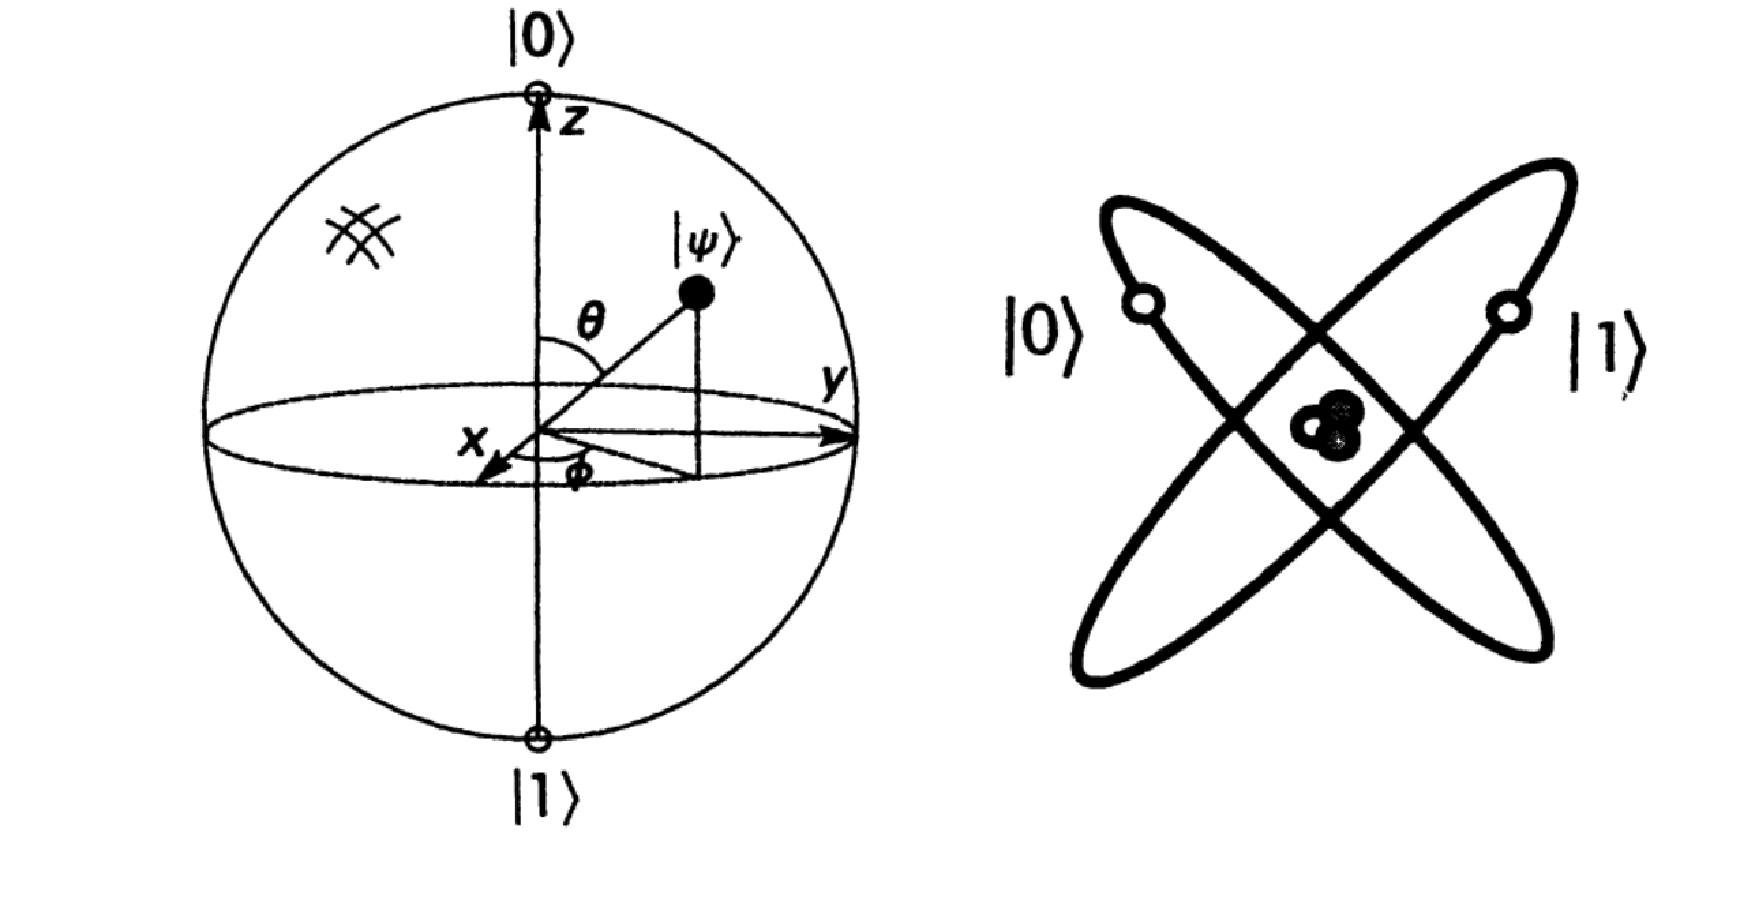
\includegraphics[width=\linewidth]{media/qubits.pdf}
    \end{figure}
	\end{frame}


    \begin{frame}{Принцип работы ионной ловушки}
    \framesubtitle{Доплеровское охлаждение}

        \begin{columns}

        \begin{column}{0.5\textwidth}

            \begin{itemize}
                \item[1.] <1-> Покоящийся атом, смещения по частоте нет, налетающий фотон
                               не поглощается
                \item[2.] <2-> Атом движется. Смещение по частоте в область красного спектра,
                               поглощение фотона не происходит
                \item[3.1] <3-> Атом движется. Смещение по частоте в область синего спектра,
                                происходит поглощение фотона.
            \end{itemize}

        \end{column}

        \begin{column}{0.5\textwidth}
            \begin{figure}
                \centering
                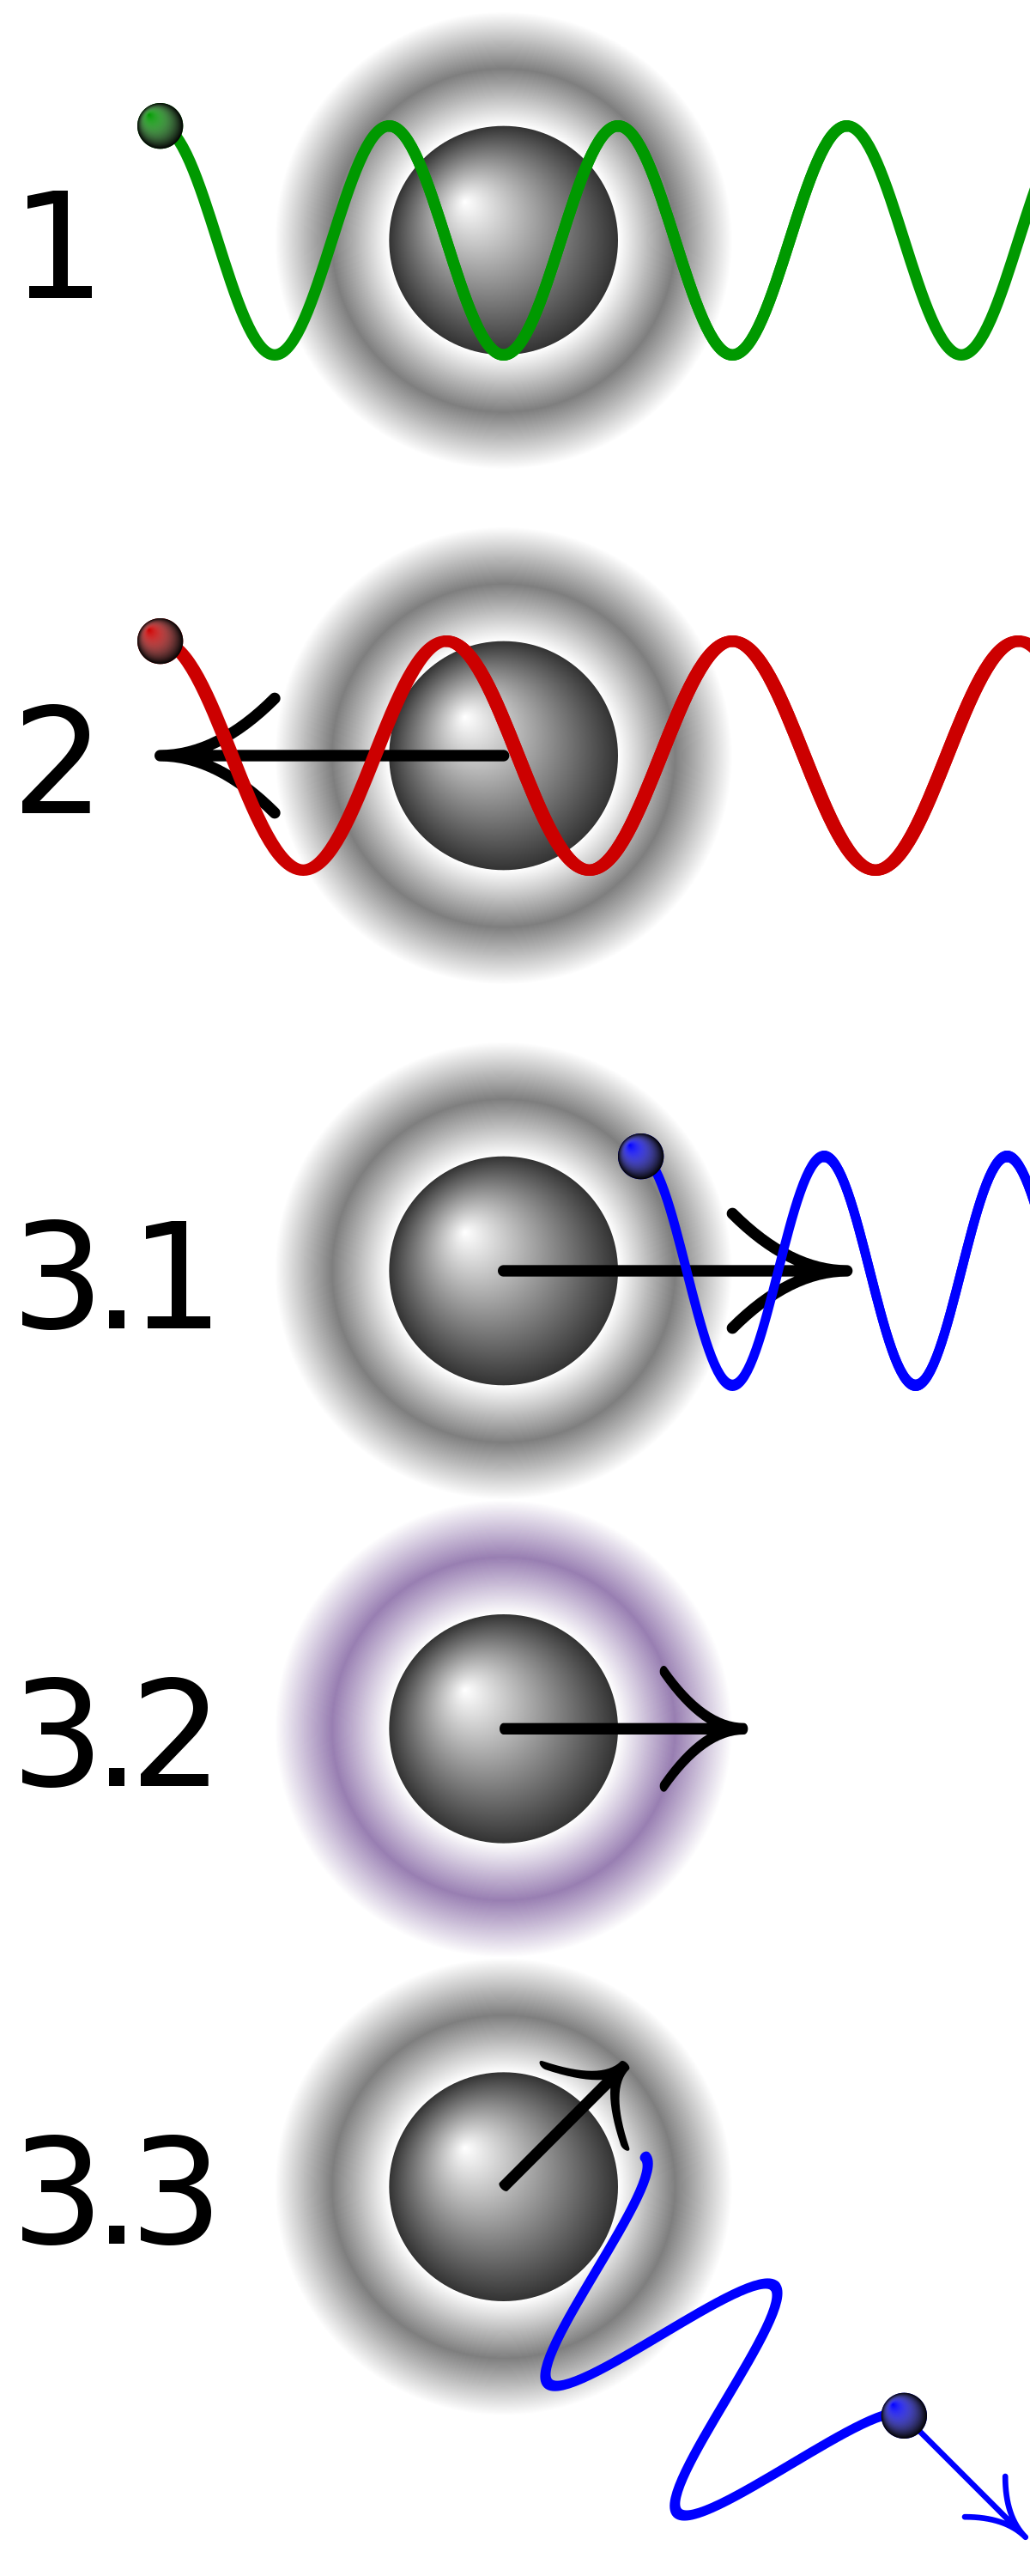
\includegraphics[width=0.35\textwidth]{media/dopler-cooling.png}
                \caption{Иллюстрация доплеровского охлаждения}
            \end{figure}
        \end{column}

        \end{columns}
    \end{frame}

    \begin{frame}{Принцип работы ионной ловушки}
    \framesubtitle{Доплеровское охлаждение}
        \begin{columns}

        \begin{column}{0.5\textwidth}

            \begin{itemize}
                \item[3.2] <1-> Атом возбуждается
                \item[3.3] <2-> Атом излучает в случайном направлении
            \end{itemize}

        \end{column}

        \begin{column}{0.5\textwidth}
            \begin{figure}
                \centering
                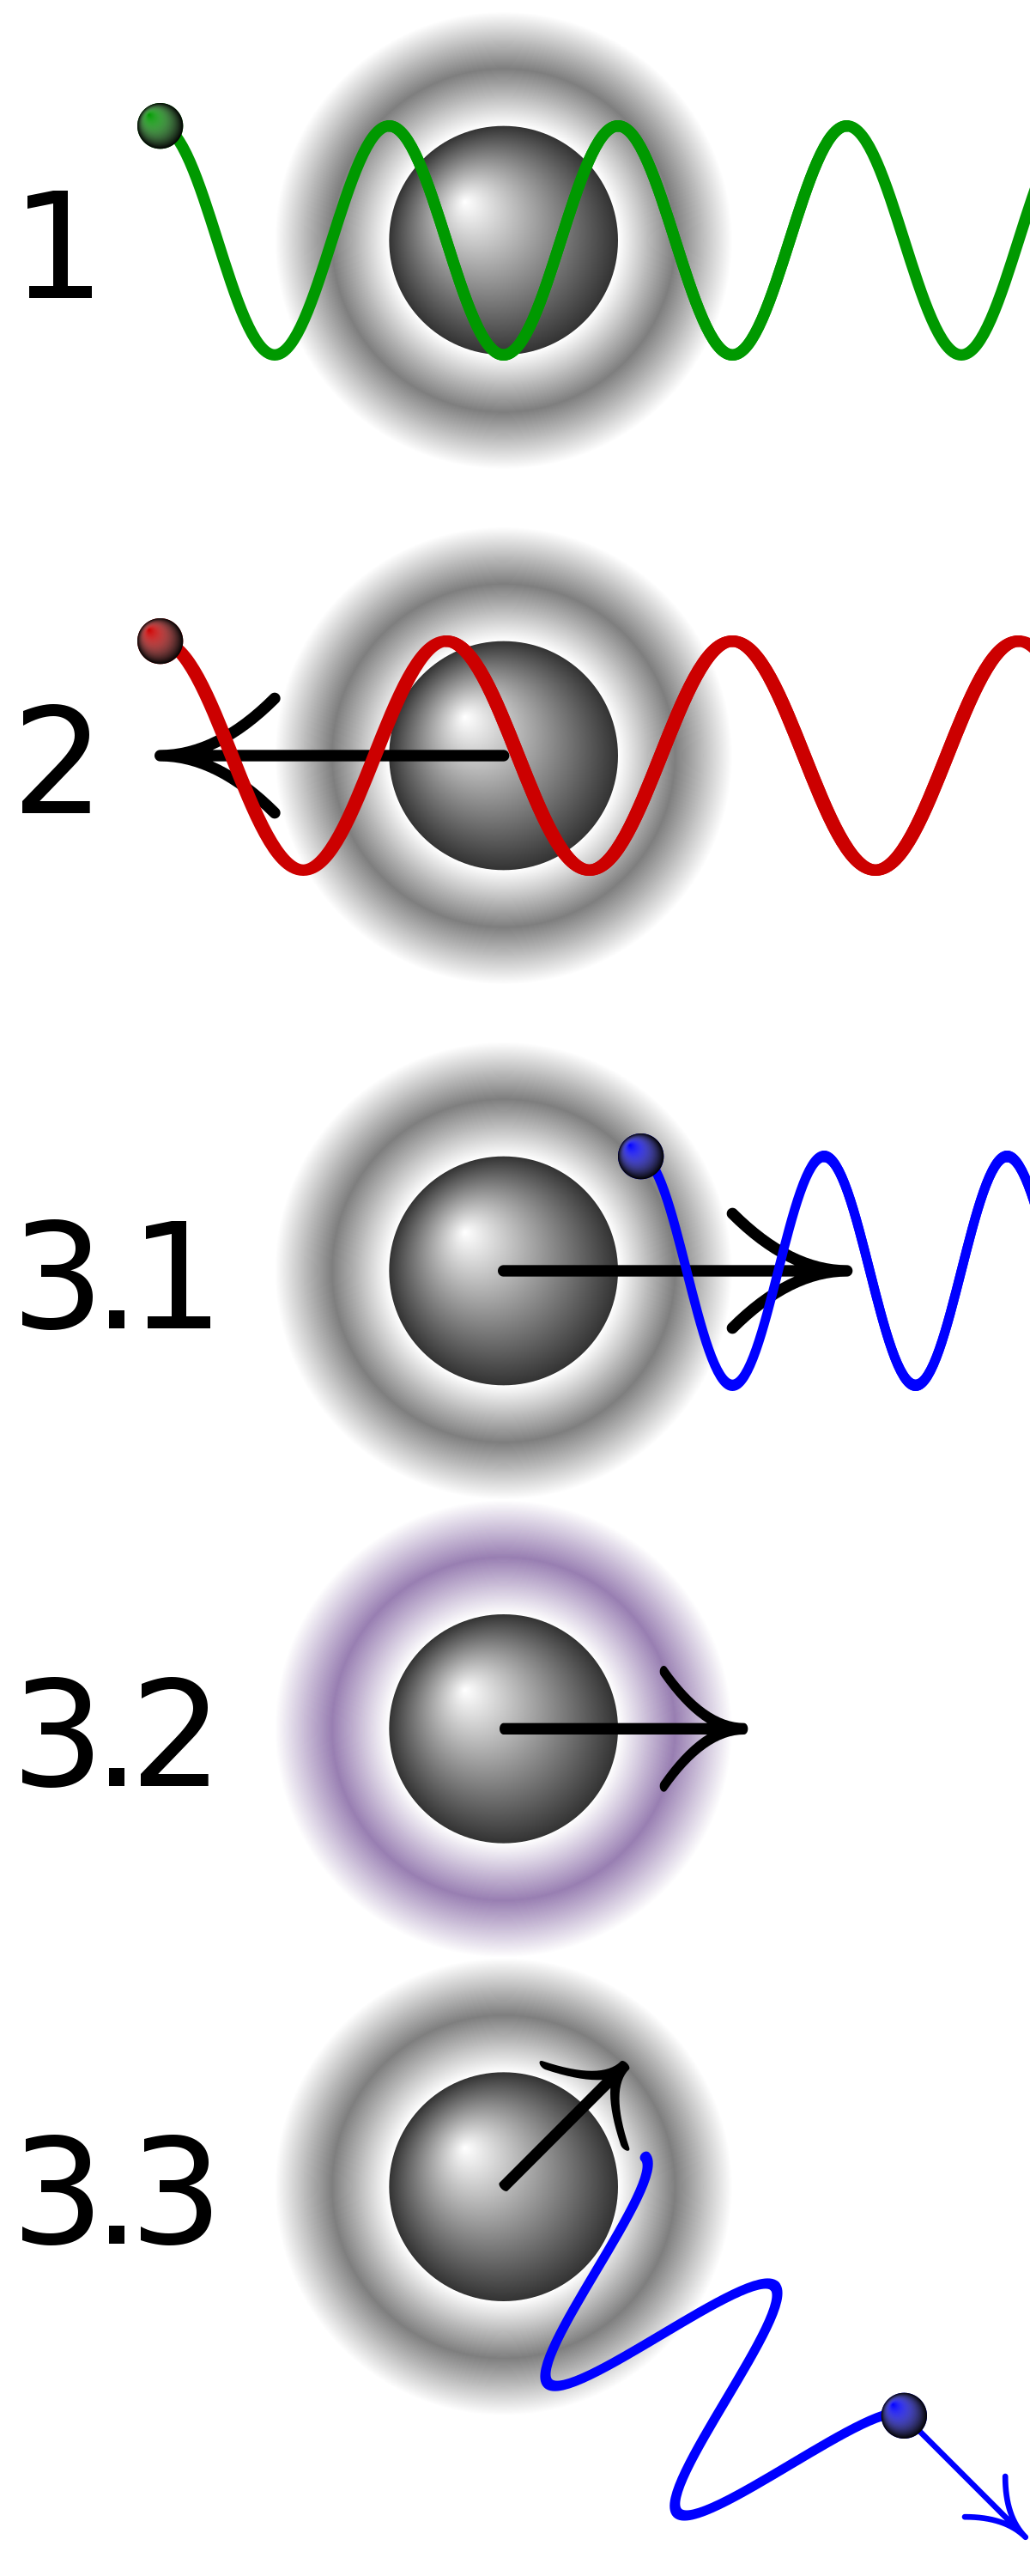
\includegraphics[width=0.35\textwidth]{media/dopler-cooling.png}
                \caption{Иллюстрация доплеровского охлаждения}
            \end{figure}
        \end{column}

        \end{columns}

    \end{frame}

    \begin{frame}{Реализация свойств квантового компьютера}
    \framesubtitle{Представление кубита}

        \begin{columns}

        \begin{column}{0.6\textwidth}

            \begin{itemize}
                \item <1-> Кубит представляет собой атомные состояния сверхтонкой структуры удерживаемых в ловушке атомов. 
                \item <2-> Два сверхтонких уровня основного состояния (они называются «сверхтонкими кубитами»)
                \item <3-> Уровень основного состояния и возбужденный уровень (они называются «оптическими кубитами»)
            \end{itemize}

        \end{column}

        \begin{column}{0.4\textwidth}
            \begin{figure}
                \centering
                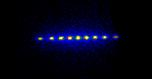
\includegraphics[width=0.35\textwidth]{media/nine-calcium-ions.jpg}
                \caption{Девять атома кальция в ловушке}
            \end{figure}
        \end{column}

        \end{columns}
    \end{frame}

    \begin{frame}{Реализация свойств квантового компьютера}
    \framesubtitle{Приготовление начального состояния}

    \begin{itemize}
            \item <1-> Состояния ионных кубитов могут быть приготовлены в определенном состоянии кубита с помощью процесса, называемого \textbf{оптической накачкой}. В этом процессе лазер связывает ион с некоторыми возбужденными состояниями, которые в конечном итоге распадаются до одного состояния, которое не связано с лазером.
            \item <2-> Как только ион достигает этого состояния, у него нет возбужденных уровней, с которыми можно было бы взаимодействовать в присутствии этого лазера, и, следовательно, он остается в этом состоянии.
    \end{itemize}


    \end{frame}

    \begin{frame}{Реализация свойств квантового компьютера}
    \framesubtitle{Приготовление начального состояния}

    \begin{itemize}
            \item <1-> Если ион распадается до одного из других состояний, лазер будет продолжать возбуждать ион до тех пор, пока он не распадется до состояния, которое не взаимодействует с лазером. Этот процесс инициализации является стандартным для многих физических экспериментов и может выполняться с очень высокой точностью (> 99,9)
    \end{itemize}

    \end{frame}

    \begin{frame}{Оптическая накачка}
    \framesubtitle{Реализация свойств квантового компьютера}

        \begin{itemize}
            \item <1-> О
        \end{itemize}

    \end{frame}


\end{document}
